\documentclass[a4paper]{report}
\usepackage{graphicx}
\usepackage{color}
%% Replace serif font with (postscript) helvetica
%\usepackage[scaled]{helvet}
\renewcommand*\familydefault{\sfdefault} %% Only if the base font of the document is to be sans serif
\usepackage[T1]{fontenc}
\setlength{\textwidth}{160mm}
\setlength{\oddsidemargin}{0mm}
\setlength{\evensidemargin}{0mm}
\setlength{\textheight}{250mm}
\setlength{\voffset}{-20mm}
%\usepackage{showframe}
\usepackage{xspace}
%\usepackage{pgffor}

\usepackage{draftwatermark}
\SetWatermarkText{DRAFT}
\SetWatermarkScale{4}
\SetWatermarkLightness{0.92}



%%%  Various reserved words  %%%
%\newcommand{\urd}{\texttt{urd}\xspace}
\newcommand{\joblist}{\texttt{JobList}\xspace}
\newcommand{\jobtuple}{\texttt{JobTuple}\xspace}
%\newcommand{\callmethod}{\texttt{call\_method}\xspace}
%\newcommand{\arecord}{\texttt{a.record}\xspace}
%\newcommand{\automatacommon}{\texttt{automata\_common}\xspace}
%\newcommand{\defaultdict}{\texttt{defaultdict}\xspace}
%\newcommand{\jobid}{\texttt{jobid}\xspace}
\newcommand{\jobids}{\texttt{jobids}\xspace}
\newcommand{\datasets}{\texttt{datasets}\xspace}
\newcommand{\options}{\texttt{options}\xspace}
\newcommand{\prepare}{\texttt{prepare}\xspace}
\newcommand{\analysis}{\texttt{analysis}\xspace}
\newcommand{\synthesis}{\texttt{synthesis}\xspace}
\newcommand{\analysisres}{\texttt{analysis\_res}\xspace}
\newcommand{\prepareres}{\texttt{prepare\_res}\xspace}
\newcommand{\params}{\texttt{params}\xspace}
\newcommand{\jobparams}{\texttt{job\_params}\xspace}
\newcommand{\sliceno}{\texttt{sliceno}\xspace}
% \newcommand{\jobids}{\texttt{jobids}\xspace}

\usepackage{xspace}
%%%  A pretty minted-environment for Python  %%%
% minted
\usepackage{minted}
\usemintedstyle{lovelace}
\definecolor{bg}{rgb}{0.95,0.95,0.95}
\definecolor{bg_shell}{rgb}{0.95,0.95,1.00}
%\newminted[python]{python}{bgcolor=bg, frame=lines}
\newminted[python]{python}{frame=lines}

\newminted[pythonBEG]{python}{frame=topline}
\newminted[pythonMID]{python}{}
\newminted[pythonEND]{python}{frame=bottomline}

\newminted[shell]{bash}{frame=lines}

\newcommand\inputfile[1]{%
    \InputIfFileExists{#1}{}{\typeout{No file #1.}}%
}

\newcommand{\exempel}[1]{\noindent\textbf{Example: #1}\\}







%\includeonly{urd}


\begin{document}

\begin{center}
  \vspace*{1.0cm}
  {\Huge The Accelerator}\\[0.7cm]
  {\Large User's Reference}
  \vspace{1.3cm}
  \begin{figure}[h]
    \centering
    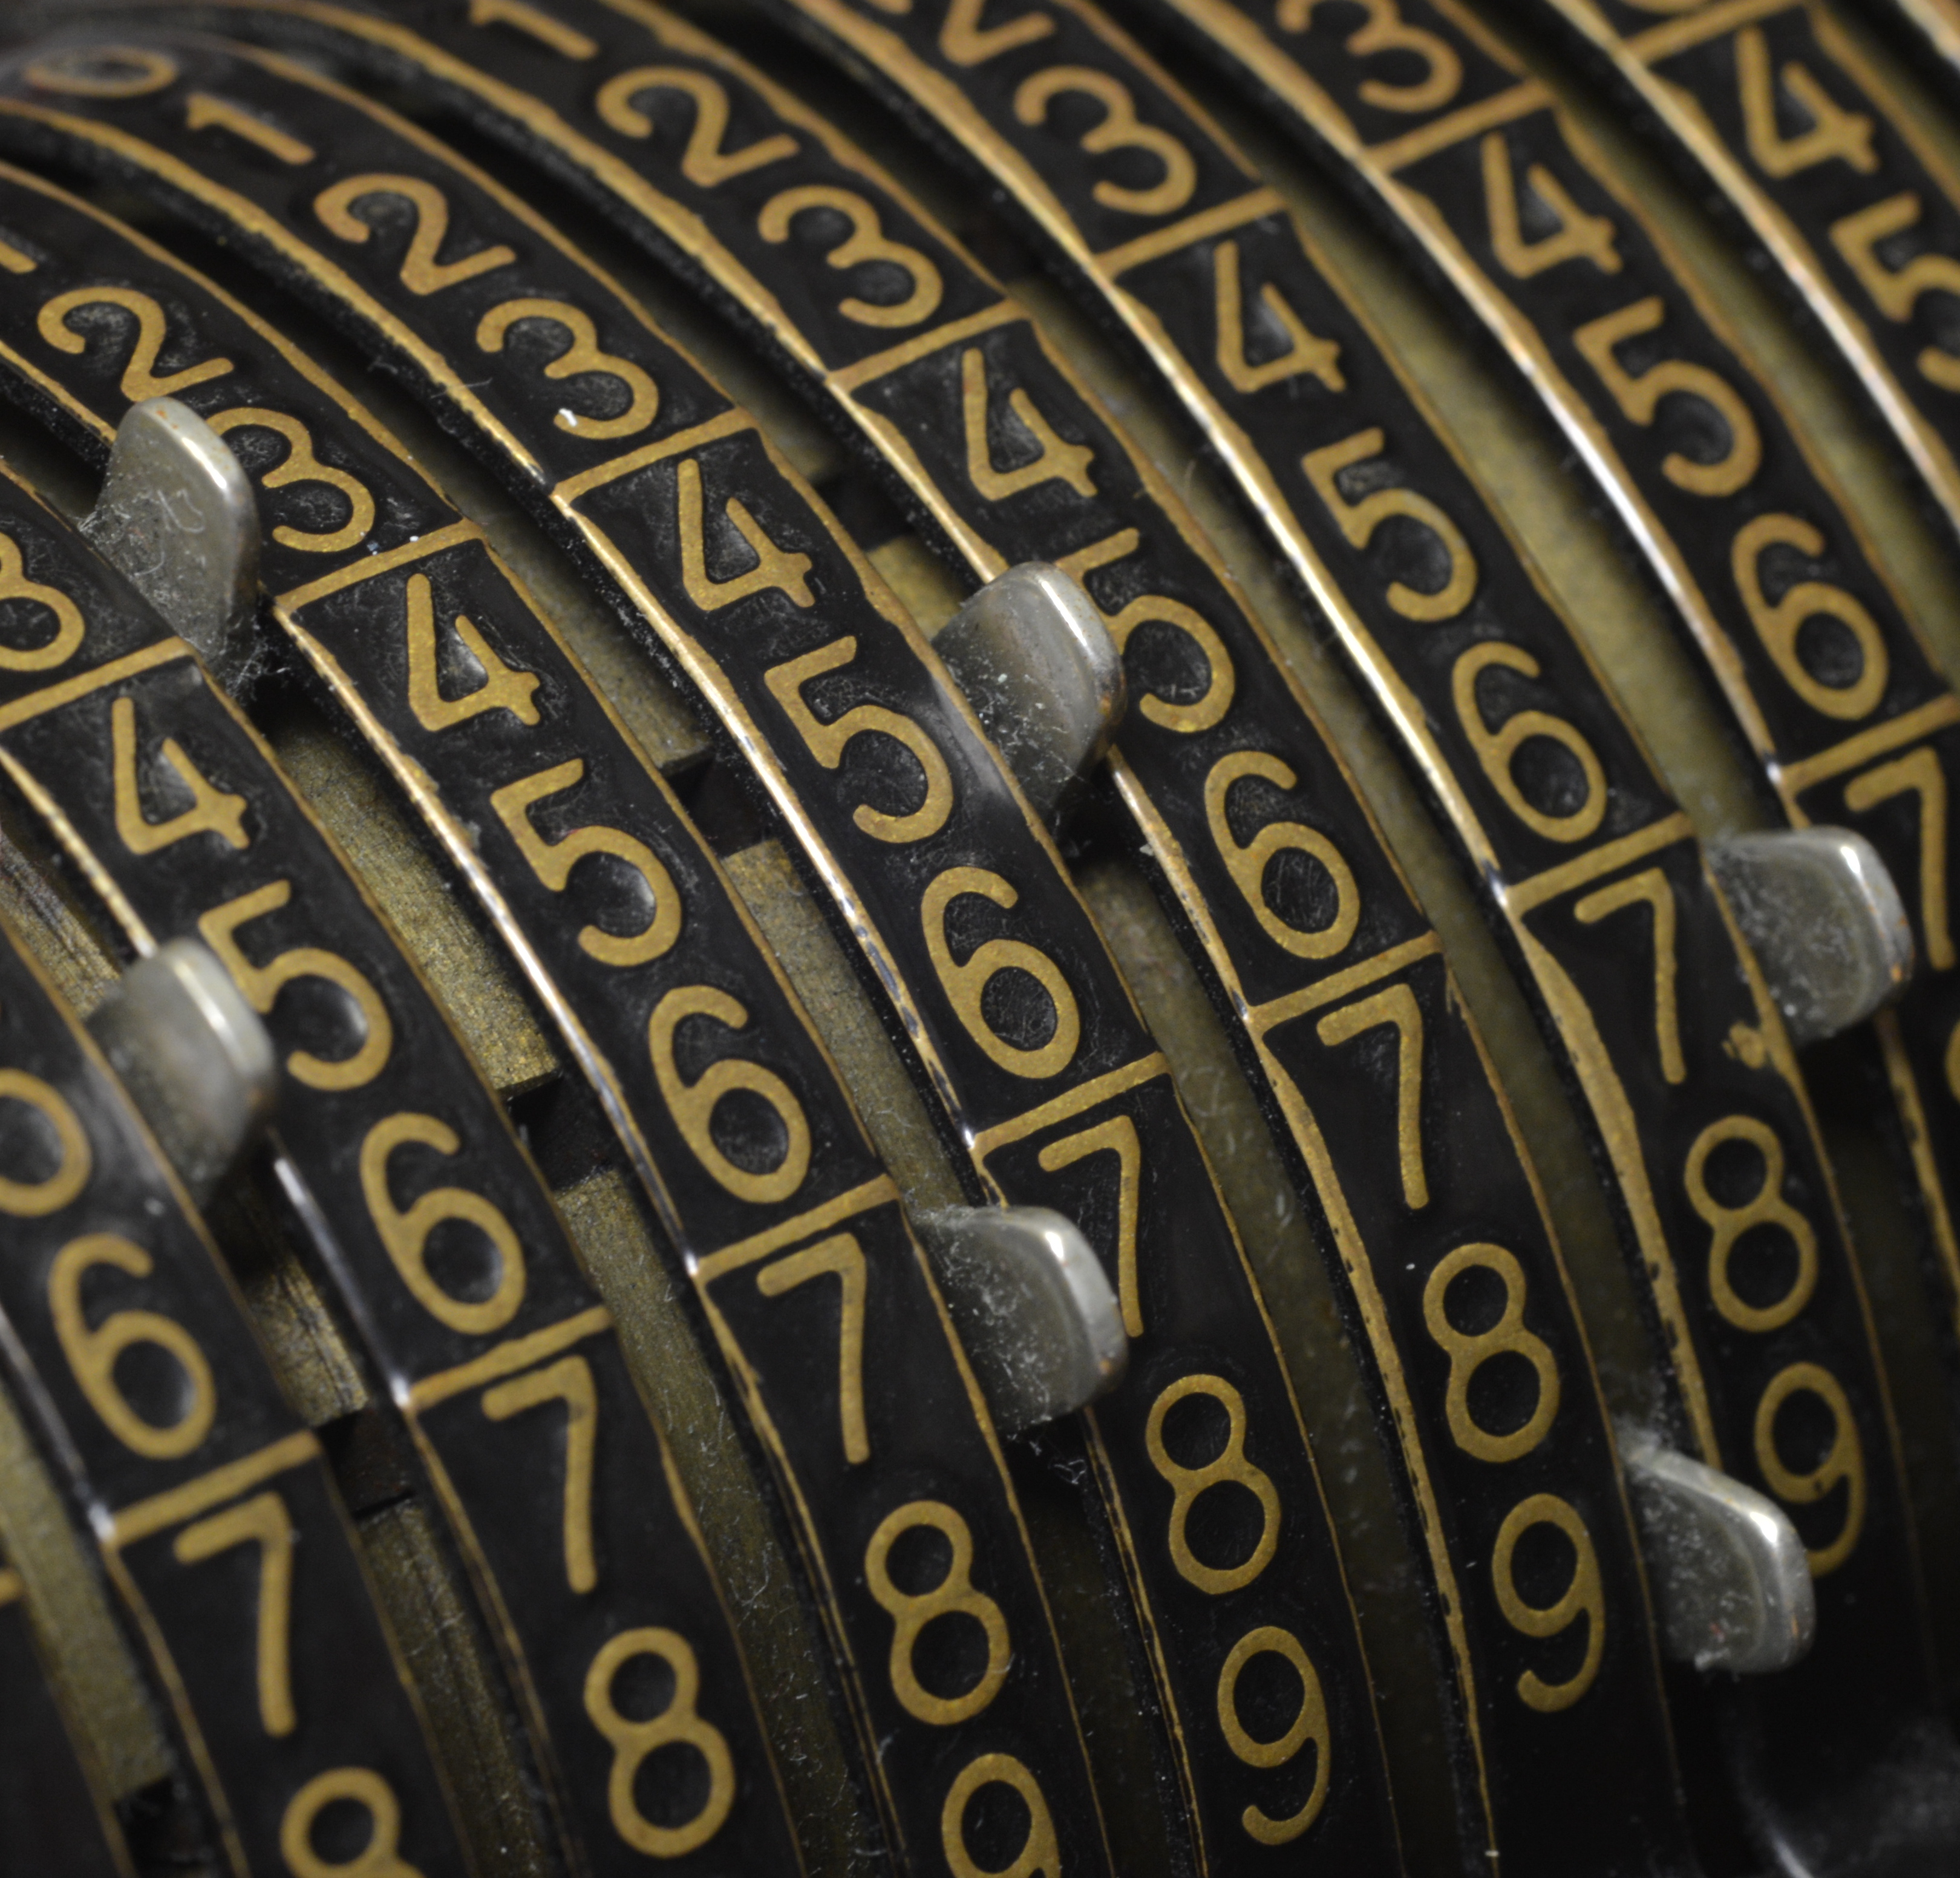
\includegraphics[width=11cm]{odhner_square.jpg}
  \end{figure}
  \vfill
  {\tiny{version: \inputfile{gitrevision}}}\\
  {\footnotesize Anders Berkeman, Carl Drougge, and Sofia H\"orberg}
\end{center}
\thispagestyle{empty}

\newpage


%\tableofcontents


\section*{Glossary}

% \begin{tabular*}{\textwidth}{l @{\extracolsep{\fill}} l}
\begin{tabular*}{\textwidth}{ll}
automata  & a script run by urd dispatching or recalling jobs\\
chain     & a one-directional list of datasets\\
dataset   & efficient storage of data\\
job       & a running or completed method\\
jobid     & a link to a successfully completed method\\
method    & main source file of program to be executed by framework\\
package   & a location where methods are stored\\
urd       & dispatcher and job database\\
workdir   & a location where job data and metadata is stored\\
\end{tabular*}


\chapter{Introduction}
%%%%%%%%%%%%%%%%%%%%%%%%%%%%%%%%%%%%%%%%%%%%%%%%%%%%%%%%%%%%%%%%%%%%%%%%%%%%
%                                                                          %
% Copyright (c) 2018 eBay Inc.                                             %
%                                                                          %
% Licensed under the Apache License, Version 2.0 (the "License");          %
% you may not use this file except in compliance with the License.         %
% You may obtain a copy of the License at                                  %
%                                                                          %
%  http://www.apache.org/licenses/LICENSE-2.0                              %
%                                                                          %
% Unless required by applicable law or agreed to in writing, software      %
% distributed under the License is distributed on an "AS IS" BASIS,        %
% WITHOUT WARRANTIES OR CONDITIONS OF ANY KIND, either express or implied. %
% See the License for the specific language governing permissions and      %
% limitations under the License.                                           %
%                                                                          %
%%%%%%%%%%%%%%%%%%%%%%%%%%%%%%%%%%%%%%%%%%%%%%%%%%%%%%%%%%%%%%%%%%%%%%%%%%%%

The Accelerator is a very efficient environment for running and
scheduling big data tasks.  It has been in continuous development
since 2012, and has been used in seven different projects, of which
three has been live to customers, and the other four was data analysis
and insight projects.

Due to its minimalistic implementation, the Accelerator is capable of
working at high speed with terabytes of data with billions of lines on
a single computer.  Two things stand out: first, all jobs are
bookkeeped in a novel way; and second, data is represented and
accessed with close to zero overhead.  The end result is a globally
optimised data processing machine with a wide spectrum of uses.

Some Accelerator features
\begin{itemize}
\item \textbf{Data integration} - The Accelerator has been used in
  several projects with different customers and data, and has thereby
  adopted to a number of formats and cases.
\item \textbf{Efficient Data Access} - Data is streamed through jobs
  using low level operating- and filesystem primitives.
\item \textbf{Simple job tracking} - Easy to find source data, easy to
  use results from other users.
\item \textbf{Transparency} - Total context for all jobs ever run is
  stored and straightforward to retreive.  Any job could be retrieved
  or replayed.
\end{itemize}






% \newpage
% Here is a list of some of the background ideas that coloured the work
% on the Accelerator.
% \begin{itemize}

% \item{parallel processing}
  
% \item \textbf{Data, recipies (code), and computation} - Data and code
%   is more important than computation.  If data integrity is
%   maintained, and code version controlled, computation is repeatable
%   and can be replicated.

% \item \textbf{Never delete or change input data} - What is saved by
%   freed storage is nothing compared to the cost of loss of history:
%   replication becomes impossible, as well as certain analyses.

% \item \textbf{Data should be accessable with minimum overhead}

% \item \textbf{Appending columns and rows should have minimal overhead.}

% \item \textbf{Live and dev environment is equivalent}
% \item \textbf{ blah - analysis and production same blah@@@}
  
% \item \textbf{Bookkeep intermediate results.  Use it --- don't recompute!}

% \item \textbf{client server configuration}

% \item \textbf{simplicity} use basic file systems, and simple,
%   minimalistic programs.  (Maintainability, stability, observability,
%   and speed).  Adding layers and applications slows things down.

% \item \textbf{Moore's law and bottlenecks} CPU, memory size, and disk
%   storage increase exponentionally over time for constant price.
%   Interconnection speed does not.  Avoid bottlenecks!

% \item \textbf{Avoid clusters} Are clusters for speed or redundancy?
%   How many machines does a cluster need to have to par a single
%   machine with data and code stored locally?
% \end{itemize}




\chapter{Overview}

\section{Introduction}

The accelerator environment is composed of two parts: a server
providing a set of features for efficient processing of large amounts
of data, and a client that dispatches jobs on the server.

A user may use or write two kinds of programs for the enviromnent.
the first is called methods, which is parallel programs executed by
the server.  The second is high level scripts, called automatas, that
are executed by the client.  Automatas are used to control flow and
parameters to and from the methods running on the server.

Programs are written in the Python programming language, both python 2
and 3 are supported.  In theory, any language may be used.

Methods that have been running are called jobs.  The server stores
results and parameters from all jobs in a database that is partitioned
into what is called workdirs.  The client keeps a log, called the urd
log, which is bookkeeping all dispatched jobs and parameters.

@@@ featurelist here?!

A very simple example

\begin{python}
# a_helloworld.py:
def analysis(sliceno):
  print("Hello world: %d" % (sliceno,))

# automata.py:
def main(urd):
  urd.begin('test')
  urd.build('helloworld')
\end{python}


\section{Job Bookkeeping}

A promiment feature of both the client and the server is the ability
to immediately recall instead of recompute previously executed jobs.
Any job that has been successfully executed may be recalled, provided
that the job is submitted again with exactly the same input and source
code.  The framework uses a hash of the method's source code to decide
if it has changed or not.

The combination of bookkeeping and the client/server architecture
provides a very powerful environment for accessing and depending on
previous result.  Not only can a user's own results be recalled, but
also those from another user or from the ``production'' user in a live
enviroment.

In a typical application, this dramatically increases performance
while minimising the probability of errors.  It also allows for a high
level of transparency.  Past jobs could be replayed in a controlled
manner, and the complete context with respect to input argments of any
job could be retreived and used to answer ``what-if''-scenarios.

@@ Jag vill inte ha exempel, utan harda definitioner!



\section{Urd}

Urd provides a scripting environment for running and recalling jobs.
It has a transaction-log database that stores information about jobs
that have been run and their inter-dependencies.

Urd is designed to answer questions like: ``what is the jobid of the
job that ran customer recommendations on this and this date'', and
``what data did that recommendation job depend on, which was the
latest available transaction log at that time''.




\section{Workdirs}

A workdir is where results are stored.  One can think of it as a
directory populated with jobid-directories.  Workdir are specified
with absolute paths in the server filesystem.  A workdir has a fixed
slicing.  All workdir in a project need to have the same number of
slices.



\section{Dispatch, Dependencies, and Jobids}

The framework is basically a job dispatcher and depencency tracker.
Input to a job is parameters and source code, called method.  When a
job is run, a directory is created in the workdir.  A pointer to this
directory, called a jobid, is returned upon finished execution.
Inside the directory, everything needed to run the job is stored, for
example input parameters, as well as all results created during
execution.

The framework keeps information for each job that has been
successfully completed for dependency tracking.  Dependency tracking
is used for two things: first, it avoids re-execution of jobs that
have been run before; and second, it permits jobs to depend on already
finished jobs.

Re-execution is avoided if a job is issued with exactly the same
source code and input options.  If source code is not equal, or if any
input to the job is different, the job will be executed again.  All
successful runs of a job will be kept.

A job may have reference to other jobs as input.  If these references
are valid, the running job will have access to all information from
the reference jobs.



\section{Datasets and Chaining}

A particularly efficient way to store data is by using the dataset.
Data is stored so that it can be retrieved row by row at a very high
pace and requesting from one to any number of columns.

Data in a dataset is separated into slices, where on a single server,
the number of slices is close to the number of actual CPU cores for
best performance.

A dataset may be hashed on one of its columns.  Hashing means that
each slice contains a mutually exclusive set of column data.

Typically, a dataset is created for each file that is imported.  When
several files are imported, the jobids may be chained, that is, each
new jobid contains a pointer to the previous job.  Using the
previous-pointers, datasets could be iterated one after another
without interruption.



\section{Method}

Code is executed on the framework is written in methods.  Methods
allow for parallel execution and more.

\section{Automata}



\chapter{High Level Control:  Urd}
\section{Introduction to Urd}

Urd is the key controller in the framework.  It is the primary job
dispatcher as well as the bookkeeper of all jobs executed.  Events in
urd are quantified into what is called \textsl{sessions}, and the core
of urd is a transaction log database storing these sessions together
with meta information.  The result is a server providing lookups for
all jobs executed together with their context.

The Urd database is partitioned into what is called \textsl{lists}.
Each user, human or agent, owns one or more lists where information
about executed jobs are stored.  Lists are globally readable, but
writing is limited using authentication, so that, for example, only
the production user may publish a model to go live.

With the exception of experimental work, all work initiated by urd is
run in closed sessons, with well defined starting and ending points.
The input dependencies to these sessions are recorded, together with
the resulting output.



\section{Urd sessions}

Here is an example of a minimal urd session
\\
\begin{python}
def main(urd):
  urd.begin('test')
  ...
  urd.finish('test', '20161025')
\end{python}
\\
Everything dispatched between \texttt{begin} and \texttt{finish} will
be appended to the \texttt{test} urd list with timestamp
\texttt{20161025}, as log as the \texttt{finish} function is called,
since it is responsible for updating the urd transaction log.  Before
\texttt{finish}, noting is stored, and it is perfectly ok to omit
\texttt{finish} during development work.

There are a number of options associated with a session, as shown
here,
\\
\begin{python}
  urd.begin(path, timestamp=None, caption=None, update=False)
  urd.finish(path, timestamp=None, caption=None)
\end{python}
\\
and the following rules apply to these options:
\begin{itemize}
  \item the same \texttt{path} must be specified in both \texttt{begin} and \texttt{finish}.
  \item \texttt{timestamp} is mandatory, but could be set in either \texttt{begin} or
    \texttt{finish}.  \texttt{finish} overrides \texttt{begin}.
  \item \texttt{caption} is mandatory, but could be set in either \texttt{begin} or
    \texttt{finish}.  \texttt{finish} overrides \texttt{begin}.
\end{itemize}
There is also an \texttt{update} option that will be discussed in
section~\ref{update_info}.



\subsubsection{Timestamp resolution}

Timestamps may be specified in various resolution depending on the
application.  The following examples cover the available formats
\\
\begin{python}
   '20161025'              day resolution
   '20161025 15'           hour resolution
   '20161025 1525'         minute resolution
   '20161025 152500'       second resolution
\end{python}



\subsubsection{Aborting an Urd Session}

When a session is initiated, a new session cannot start until the
current has finished.  A session may be aborted, however,
\\
\begin{python}
  urd.begin('test')
  urd.abort()
\end{python}
\\
and aborted sessions are not stored in the urd transaction log.



\newpage
\section{Building jobs}

Jobs are dispatched in session using the \texttt{build} function.  The
syntax is as follows
\\
\begin{python}
  jobid = urd.build('method1', options={}, datasets={}, jobids={}, ...)
\end{python}
\\
where \texttt{options}, \texttt{datasets}, and \texttt{jobids} are
optional, depending on the method to be dispatched.  In addition, a
name and a caption may optionally be specified too
\\
\begin{python}
  jobid = urd.build('method1', name='myjob', caption='looking for something')
\end{python}
\\
The name will replace the method name in the joblist, in this case,
this job will now be referred to as \texttt{myjob} (default was
\texttt{method1}).  A jobid to the finished job is returned upon
successful completion.





\subsection{Building chained jobs}
It is also possible to build chained jobs implicitly using the
\texttt{build\_chained} function
\\
\begin{python}
  jobid = urd.build_chained('method1', name='myjob')
\end{python}
\\
which takes the same options as the standard \texttt{build} method,
with the exception that name is mandatory, since it is used to find
the previous job of matching type.



\subsection{Debug:  Why build}

By specifying the flag \texttt{why\_build} to the automatarunner it is
possible to see the reasons for building a job.  For example
\\
\begin{python}
  print(urd.build('method3', jobids=dict(firstjob=jid2, secondjob=jid2), name='knut'))
# Would have built from:
# ======================
# {
#     "caption": "fsm_method3", 
#     "method": "method3", 
#     "params": {
#         "method3": {
#             "datasets": {}, 
#             "jobids": {
#                 "firstjob": "test-59_0", 
#                 "secondjob": "test-59_0"
#             }, 
#             "options": {}
#         }
#     }, 
#     "why_build": "on_build"
# }
# Could have avoided build if:
# ============================
# {
#     "method3": {
#         "test-60_0": {
#             "jobids": {
#                 "firstjob": "test-56_0"
#             }
#         }
#     }
# }
\end{python}
\\
A more machine-friendly output is possible by spefifying
\texttt{why\_build=True} in the \texttt{build}-request (and not
specifying it to the automatarunner).



\newpage
\section{Sessions with dependency}

A job may have dependencies, such as other jobs or datasets.  These
dependencies are input to the job using the corresponding arguments to
the \texttt{build} function.  Locating these jobs or datasets,
however, is exactly a design goal of Urd.  Urd implements a
\texttt{get} function that looks up jobids and dependencies from a key
that is composed of a urd list name and a timestamp.  There are also,
for convenience, \texttt{first} and \texttt{latest} functions to get
the first and latest job in an urd list.

Here is an example.  Assume that a method, \texttt{method1}, uses some
kind of imported transaction logs, called \texttt{tlog}.  When
dispatching \texttt{method1}, it should be using the latest available
\texttt{tlog}.  The example shows how the function \texttt{latest} is
used for this
\\
\begin{python}
def main(urd):
  urd.begin('test')
  latest_tlog = urd.latest('tlog').joblist.jobid
  urd.build('method1', datasets=dict(tlog=latest_tlog))
  urd.finish('test', '20161025')
\end{python}
\\
Two things have happened here.  First, urd has provided a jobid link
to the latest available \texttt{tlog}.  Second, the dependency of
exactly this version of \texttt{tlog} to \texttt{method1} is recorded
in the urd list \texttt{test} for timestamp \texttt{20161025}.  So, if
there is a question in the future which version of the \texttt{tlog}
database that was used on that date for the \texttt{method1} function,
it is immediately available from urd.

The more general form is \texttt{get}, which is shown below together
with its derived convenience-functions
\\
\begin{python}
  urd.get('test', '20161001')
  urd.latest('test')
  urd.first('test')
\end{python}
\\
And here is an example of running \texttt{method1} on \texttt{tlog} data
from previous month
\\
\begin{python}
def main(urd):
  urd.begin('test')
  tlog = urd.get('tlog', '20160925').joblist.jobid
  urd.build('method1', datasets=dict(tlog=tlog))
  urd.finish('test', '20161025')
\end{python}



\section{Avoiding recording dependency}
Depencency-recording will be activated on use of the \texttt{get},
\texttt{latest}, and \texttt{first} functions.  If, for some reason,
the point is to just have a look at the database to see what is in
there, it can be done using the peek-versions, as presented below:
\\
\begin{python}
  urd.peek('test', '20161025')
  urd.peek_latest('test')
  urd.peek_first('test')
\end{python}



\newpage
\section{More on Finding Items in Urd}
There is a \texttt{list} function that returns what lists are recorded
in the database:
\\
\begin{pythonBEG}
  print(urd.list())
  # ['ab/test', 'ab/live']
\end{pythonBEG}
\\
And there is also a \texttt{since} function that returns a list of all
timestamps after the input argument
\\
\begin{pythonMID}
  print(urd.since('20161005'))
  # ["20161006", "20161007", "20161008", "20161009"]
\end{pythonMID}
\\
The \texttt{since} is rather relaxed with respect to the resolution of
the input.  The input timestamp may be truncated from the right down
to only one digits.  An input of zero is also valid.
\\
\begin{pythonEND}
  print(urd.since('0'))
  # ["20160101", "20161004", "20161005", "20161006", "20161007", "20161008"]
  print(urd.since('2016'))
  # ["20160101", "20161004", "20161005", "20161006", "20161007", "20161008"]
  print(urd.since('20161'))
  # ["20161004", "20161005", "20161006", "20161007", "20161008"]

  print(urd.since('2016105'))
  # ["20161006", "20161007", "20161008"]
  ...
  print(urd.since('2016105 000000'))
  # ["20161006", "20161007", "20161008"]
\end{pythonEND}



\section{Truncating and Updating}

Urd will always keep a consistent history of all events taken place.
Sometimes, however, it makes sense to re-run events from the past.
There are two means to achieve this, update and truncate.

\subsubsection{update}
The begin-function takes an optional argument update

\begin{python}
  urd.begin('test', '20161025', update=True)
\end{python}
\\
If update is True, the entry in the test list at '20161025' will be
updated, unless there has been no change.

\subsubsection{Truncate}

The truncate() class member is used to rollback an arbitrary amount of
an urd list.

\begin{python}
  urd.truncate('test', '20160930')
\end{python}
\\
This will rollback everything that has happened in the test list back
to '20160930'.  Internally, urd stores the complete history, however.



\newpage
\section{More on Joblist and Jobtuple}

Urd is using the type joblist to keep track of successfully executed
jobs.  Each item in the joblist is of type jobtuple.  This section
will start by describing jobtuple first and then joblist.

\subsubsection{Jobtuple}

The \jobtuple type is used to group method names and corresponding
jobids.  It is basically a tuple with some extra properties, such as a
conversion of a jobtuple to \texttt{str}, which happens for example
when printing it, returns the jobid as a string.

\begin{pythonBEG}
>>> jt = JobTuple('imprt', 'jid-0_0')

>>> jt
('imprt', 'jid-0_0')
\end{pythonBEG}
\\
as expected, and

\begin{pythonMID}
>>> jt.method
'imprt'

>>> jt.jobid
'jid-0_0'
\end{pythonMID}
\\
but note that

\begin{pythonEND}
>>> print(jt)  # str and encode return jobid only
jid-0_0
\end{pythonEND}



\subsubsection{JobList}

\label{sec:joblist}
The \joblist is a list with add-ons for bookkeeping and finding jobs.
It stores instances of \jobtuple.  Here is an example.  First, define
a \jobtuple

\begin{pythonBEG}
>>> jt = JobTuple('imprt', 'jid-0_0')
\end{pythonBEG}
\\
then define a joblist initiated with the same tuple.  Then append some
more jobs directly using the \texttt{append} method.

\begin{pythonMID}
>>> jl = JobList(jt)
>>> jl.append('learn', 'lrn-0_0')
>>> jl.append('imprt', 'imp-1_0')
\end{pythonMID}
\\
Let's see how and what is stored in the \joblist.  The \texttt{pretty}
method is quite useful, but note that just printing the object will
show the last jobid only.

\begin{pythonMID}
>>> print(jl.pretty)
JobList(
   [  0]  imprt : jid-0_0
   [  1]  learn : lrn-0_0
   [  2]  imprt : imp-1_0
)

>>>  print(jl)  # jobid of latest appended JobTuple
imp-1_0
\end{pythonMID}

It is easy to retreive the last job with a particular \texttt{method}
name, either by lookup or by using \texttt{find}.

\begin{pythonMID}
>>> jl['imprt']         # latest jobid with name 'imprt'
('imprt', 'imp-1_0')

>>> print(jl['imprt'])   # jl['imprt'] is JobTuple
imp-1_0
\end{pythonMID}
\\
The Find method returns a \joblist.  Slicing also returns {\joblist}s

\begin{pythonMID}
>>> jl.find('imprt')
JobList([('imprt', 'jid-0_0'), ('imprt', 'imp-1_0')])

>>> jl[:2]
JobList([('imprt', 'jid-0_0'), ('learn', 'lrn-0_0')])
\end{pythonMID}
\\
Looking up by index returns \jobtuple.

\begin{pythonMID}
>>> jl[0]
('imprt', 'jid-0_0')
\end{pythonMID}
\\
These conveniences are also supported

\begin{pythonEND}
>>> jl.all              # list of all jobids
'jid-0_0,lrn-0_0,imp-1_0'

>>> jl.method           # last method
'import'

>>> jl.jobid            # last jobid
'imp-1_0'
\end{pythonEND}



\newpage
\section{Urd HTTP\_API}

In some situations it is convenient to make calls to urd directly
without using the framework.  Urd will react to HTTP requests.

\begin{shell}
% curl http://localhost:8833/list
["ab/test"]

% curl http://localhost:8833/ab/test/latest
{"caption": "", "automata": "test", "user": "ab", "deps": {},
  "timestamp": "20161025", "joblist": [["method1", "test-56_0"],
  ["method2", "test-59_0"], ["method3", "test-60_0"]]}

% curl http://localhost:8833/ab/test/first
{"caption": "", "automata": "test", "user": "ab", "deps": {},
  "timestamp": "20161025", "joblist": [["method1", "test-56_0"],
  ["method2", "test-59_0"], ["method3", "test-60_0"]]}

% curl http://localhost:8833/ab/test/20161025
{"caption": "", "automata": "test", "user": "ab", "deps": {},
  "timestamp": "20161025", "joblist": [["method1", "test-56_0"],
  ["method2", "test-59_0"], ["method3", "test-60_0"]]}

% curl http://localhost:8833/ab/test/since/201610024
["20161025"]
% curl http://localhost:8833/ab/test/since/20161026
[]                                 
\end{shell}


\chapter{Method}
\section{Method inputs}

There are three kinds of input to a method
\begin{itemize}
\item options
\item datasets
\item jobids
\end{itemize}

each vill be described in more detail next

\subsection*{options}
The options is of type dict.  Example

\begin{python}
from extras import OptionEnum, JobWithFile
options = dict(
  length = 1,
  colname = "gtin",
  operation = OptionEnum("lt le gt ge").ge,
  datafile = JobWithFile,
)
\end{python}
In the example above, the following happens
\begin{itemize}
\item length is typed to int, and default value is 1.
\item colname is typed to string, and default value is "gtin".
\item operation is one of lt, le, gt, ge, and defaults to ge.
\item datafile is more complex, for example datafile.jobid is a jobid,
  such as "pelle-123\_0", datafile.filename is a filename, such as
  "result.pickle", datafile.sliced is a boolean.  If true, the
  datafile is actually a sliced set of files, one for each target
  slice during execution, extra is what?
\end{itemize}

\subsubsection{types}
set, jobwithfile, datetime, date, time, timedelta




\subsubsection{JobWithFile}

jobid, sliced, filename, extra


\subsubsection{OptionDefault}
What?


\subsubsection{OptionString}
Marker value to specify in options\{\} for requiring a non-empty string.
You can use plain OptionString, or you can use
OptionString('example'), without making 'example' the default.
    

\subsubsection{OptionEnum}
From the source code

\begin{python}
    """A little like Enum in python34, but string-like.                                                                                                                                                                           
    (For JSONable method option enums.)                                                                                                                                                                                           
                                                                                                                                                                                                                                  
    >>> foo = OptionEnum('a b c*')                                                                                                                                                                                                
    >>> foo.a                                                                                                                                                                                                                     
    'a'                                                                                                                                                                                                                           
    >>> foo.a == 'a'                                                                                                                                                                                                              
    True                                                                                                                                                                                                                          
    >>> foo.a == foo['a']                                                                                                                                                                                                         
    True                                                                                                                                                                                                                          
    >>> isinstance(foo.a, OptionEnumValue)                                                                                                                                                                                        
    True                                                                                                                                                                                                                          
    >>> isinstance(foo['a'], OptionEnumValue)                                                                                                                                                                                     
    True                                                                                                                                                                                                                          
    >>> foo['cde'] == 'cde'                                                                                                                                                                                                       
    True                                                                                                                                                                                                                          
    >>> foo['abc']                                                                                                                                                                                                                
    Traceback (most recent call last):                                                                                                                                                                                            
    ...                                                                                                                                                                                                                           
    KeyError: 'abc'                                                                                                                                                                                                               
                                                                                                                                                                                                                                  
    Pass either foo (for a default of None) or one of the members                                                                                                                                                                 
    as the value in options{}. You get a string back, which compares                                                                                                                                                              
    equal to the member of the same name.                                                                                                                                                                                         
                                                                                                                                                                                                                                  
    Set none_ok if you accept None as the value.                                                                                                                                                                                  
                                                                                                                                                                                                                                  
    If a value ends in * that matches all endings. You can only access                                                                                                                                                            
    these as foo['cde'] (for use in options{}).                                                                                                                                                                                   
    """
\end{python}

\subsection{datasets}
datasets is the way to communicate datasets from automata to job.  In
the running method, the datasets variable is a list of dataset objects
ready to use.

\subsection{jobids}
the jobids argument is a tuple of jobids linking this job to other
jobs.  jobids is different from datasets in that jobids does not
contain any dataset jobs.  Thus, no dataset objects are infered from
the jobids in the tuple.



\section{Code flow:  prepare - analysis - synthesis}

\section{More on intermediate and result files}

\subsection{Sharing data inside a job}
data is simply shared between prepare, analysis, and synthesis as follows.
\begin{itemize}
\item what is returned in prepare is available as prepare_res in analysis and synthesis
\item what is returned in analysis is available as analysis_res in synthesis.  analysis_res is an iterator.
\item what is returned in synthesis is a persistent file in the job catalog referenced by ``result''.
\end{itemize}

The simplest way to share intra job data is using the blob module.

\begin{python}
import blob
def synthesis()
  blob.load(filename')
\end{python}

saving is as follows
\begin{python}
  blob.save(data, filename, sliceno, temp)
\end{python}
sliceno and temp are optional.  If sliceno is set, data is stored in a
sliced file.  This is typically used in analysis, where each thread
will save its own file.

temp is used for file persistence.  By default, files are stored
permanently when a job terminates successfully.  Setting temp to True
removes them upon completion of the job.

Temporary files are useful when communicating data between the
functions in the method (and not using the res-files) or in debugging.

\section{debug help}
There is also a more advanced debug functionality relating to temp.

\begin{python}
from extras import Temp
def analysis(sliceno):
  ...
  blob.save(data, filename, sliceno=sliceno, temp=Temp.DEBUG)
  # or
  blob.save(data, filename, sliceno=sliceno, temp=Temp.DEBUGTEMP)
\end{python}
where the first only stores when --debug is specified, and the other
always stores but removes unless --debug is set.



\section{subjobs}


\chapter{Dataset}
%%%%%%%%%%%%%%%%%%%%%%%%%%%%%%%%%%%%%%%%%%%%%%%%%%%%%%%%%%%%%%%%%%%%%%%%%%%%
%                                                                          %
% Copyright (c) 2018 eBay Inc.                                             %
%                                                                          %
% Licensed under the Apache License, Version 2.0 (the "License");          %
% you may not use this file except in compliance with the License.         %
% You may obtain a copy of the License at                                  %
%                                                                          %
%  http://www.apache.org/licenses/LICENSE-2.0                              %
%                                                                          %
% Unless required by applicable law or agreed to in writing, software      %
% distributed under the License is distributed on an "AS IS" BASIS,        %
% WITHOUT WARRANTIES OR CONDITIONS OF ANY KIND, either express or implied. %
% See the License for the specific language governing permissions and      %
% limitations under the License.                                           %
%                                                                          %
%%%%%%%%%%%%%%%%%%%%%%%%%%%%%%%%%%%%%%%%%%%%%%%%%%%%%%%%%%%%%%%%%%%%%%%%%%%%

The Dataset class provides fast and simple access to data.  It is the
prefered way to store data using the Accelerator.  Datasets are
created by methods, and are therefore located inside job directories.
There can be any number of Datasets in a job.

The most obvious way to generate a dataset is using the
\texttt{cvsimport} method that creates a dataset from an input file.
But much more advanced use is possible since a job may contain more
than one Dataset.  Being able to create several Datasets at once
allows for efficient storage and access of data in some common
practical situations.  For example, a filtering job may split the
input Dataset into two or more output Datasets that can be accessed
independently.

For performance reasons, datasets are typically split into several
slices, where each data row exists in exactly one of the slices.  The
actual slicing may be carried out in different ways, like round robin,
or even random, but an interesting approach is to slice according to
the hash value of a certain column.  Slicing according to a hashed
column ensures that all rows with a certain column value always ends
up in the same slice.

\comment{This chapter covers ...
chaining, where datasets grows in number of lines, and column
appending, where datasets grow in number of columns.}


\section{Chaining}
When a dataset is created, it is optional to input a link to another
dataset using the parameter \texttt{previous}.  This is called
\emph{chaining}.  Chaining provides a lightweight way to append rows
to datasets, simply by linking datasets together.  A typical use case
is the import of log files.  A new dataset is created from each new
log file, and each dataset chains to the previous.  Reading the full
chain will access all log rows.  This has effect on the dataset
\emph{iterators} (see section~\ref{xx}), which may continue iterating
over the next dataset in the chain when the current dataset is
exhausted.


\section{Slicing and Hashing}
Datasets are by default sliced into a number of slices specified by
the Accelerator's configuration file~\ref{}.  Slicing means that the
rows of data in the dataset are distributed into different sets,
called slices.  Typically, there is one file on disk for each slice
and column.  The main reason for doing this is performance.  All files
could be read in parallel.  A technical detail is that if the files
become too small, all slices will be grouped into a single file which
is read by seek offset for each slice.  This will greatly improve
performance on systems with significant disk seek time.

Datasets can be sliced in a number of different ways.  A simple method
is to use round-robin, which cycles through the slices when writing.
Round-robin will balance the number of rows per slice as equal as
possible, which is a good thing in many scenarios.

Another way is to slice by looking at the values of a fixed single
column and put all rows with equal values in the same column.  This
way, data will be sliced ``by content'', and the number of rows per
slice may vary significantly.  In the context of the Accelerator, this
is called \emph{hashing}, and a dataset can be hashed on any single
column.  The advantage of this method is that data in each slice
becomes independent in many application, which is ideal for parallel
processing of the dataset.



\section{Dataset as Input Parameter}
Datasets may be input to a method using the \texttt{datasets} input
parameter list.  In a running job, the items in this list are object
of the \texttt{Dataset} class.  This class has a number of member
functions, for example
\begin{python}
datasets = ('source',)

def synthesis():
  print(datasets.source.shape)
\end{python}
will print the number of rows and columns of the \texttt{source}
Dataset.


\section{Datasets from Jobids}
Although a not so common operation, a Dataset object can be
instantiated from a jobid, like this
\begin{python}
from dataset import Dataset
...
d = Dataset('foo-0')
\end{python}
In this case, \texttt{d} will be an object based on the default
dataset residing at jobid \texttt{foo-0}.  If the dataset is stored by
a different name, it may be accessed like this
\begin{python}
d = Dataset('foo-0/bar')
# or
d = Dataset(('foo-0', 'bar'))
\end{python}







\clearpage
\section{Dataset Properties}
The Dataset class has a number of member functions and attributes that
is intended to make it simple to work with.  These functions will be
described in the next sections.


\subsection*{Column Names}
All columns in a dataset may be aquired using the \texttt{columns}
property, like this
\begin{python}
datasets = ('source',)

def synthesis():
  print(datasets.source.columns.keys())
  # may print something like
  # ['GTIN', 'date', 'locale', 'subsource']
\end{python}
The \texttt{columns} attribute is actually a dictionary from column
name to properties, as will be shown in the next section.


\subsection*{Column Properties}
For each column, the name, type, and if applicable, the minimum and
maximum values are accessible like this
\begin{python}
print(datasets.source.columns['locale'].type)
# number

print(datasets.source.columns['locale'].name)
# locale

print(datasets.source.columns['locale'].min)
# 3

print(datasets.source.columns['locale'].max)
# 107
\end{python}


\subsection*{Rows per Slice}

It may be interesting to see how many rows there are per slice in a
dataset.  This information is available as a list, for example
\begin{python}
print(datasets.source.lines)
# [5771, 6939, 6212, 6312, 6702, 6341, 5988, 6195,
#  6741, 6587, 6518, 5840, 6327, 5933, 6745, 6673,
#  6536, 6405, 6259, 6455, 6036, 6088, 6937, 6245,
#  6418, 6437, 6360, 6106, 6878]
\end{python}
The first item in the list is the number of rows in slice 0, and so
fourth.  The total number of rows in the Dataset is the sum of these
numbers.


\subsection*{Dataset Shape}
The shape of the dataset, i.e.\ the number of rows and columns, is
available from the shape attribute
\begin{python}
print(datasets.source.shape)
# (4, 184984)
\end{python}
The second number is exactly the sum of the number of lines for each
slice from above.


\subsection*{Hashlabel}
If the dataset is hashed on a particular column, the name of this
column is stored in the hashlabel attribute
\begin{python}
print(datasets.source.hashlabel)
# GTIN
\end{python}



\subsection*{Filename and Caption}
The dataset may have a filename associated to it.  This makes sense in
situations for example where the dataset is created from an input data
file using \texttt{csvimport} or similar.  The filename is accessable
using the \texttt{filename} attribute:
\begin{python}
print(datasets.source.filename)
# /data/incoming/raw_repository_5391.gz
\end{python}
Furthermore, it is possible to set a caption at dataset creation time.
The caption is entirely user-defined and has no function in the
Accelerator.  The caption is accessible like this
\begin{python}
print(datasets.source.caption)
# rehash_of_raw_data
\end{python}



\subsection*{Chains}
The previous dataset in a dataset chain is found in the
\texttt{previous} attribute:
\begin{python}
print(datasets.source.previous)
# import-4893/default
\end{python}



\newpage
\section{Column Typing}
The dataset columns are typed.  All types are shown in
table~\ref{tab:types}.  More details follow in the next sections.

\begin{snugshade}
%\begin{table}[h!]
 \begin{tabular}{p{3cm} p{8cm}}
\\
   \textbf{typename}   & \textbf{explanation} \\[2ex]\hline\\
   \texttt{number}     &  float or int\\
   \texttt{number:int} &  int\\[1ex]
   
   \texttt{float64}   &  64 bit (double) float\\
   \texttt{float32}   &  32 bit float\\
   \texttt{int64}     &  64 bit signed integer\\
   \texttt{int32}     &  32 bit integer\\[1ex]
   
   \texttt{bool}      &  True or False\\[1ex]
   
   \texttt{date}      &  date\\
   \texttt{time}      &  time\\
   \texttt{datetime}  &  complete date and time object\\[1ex]
   
   \texttt{bytes}     &  raw input, avoid \\
   \texttt{ascii}     &  ascii is faster in python2, otherwise use unicode\\
   \texttt{unicode}   &  use for strings\\[1ex]
   
   \texttt{parsed:number}   & int, float or string parsing into \texttt{number} \\
   \texttt{parsed:float64}  & int, float or string parsing into \texttt{float64} \\
   \texttt{parsed:float32}  & int, float or string parsing into \texttt{float32} \\
   \texttt{parsed:int64}    & int, float or string parsing into \texttt{int64} \\
   \texttt{parsed:int32}    & int, float or string parsing into \texttt{int32} \\[1ex]
   
   \texttt{json}            &  a datastructure that is jsonable\\
   \texttt{parsed:json}     &  string containing parseable json\\[1ex]
   
 \end{tabular}
% \caption{Available dataset column types.}
% \label{tab:types}
%\end{table}
\end{snugshade}

\comment{what are parsed:xx for?}

\subsection{Arbitrary precision numbers:  \texttt{number}}
The type \texttt{number} is integer when possible and float otherwise.
it can handle very large numbers, up to $\pm (2^{1007}-1)$.  Integers
are enforced using \texttt{number:int}, and it accepts trailing
decimal zeroes like \texttt{7.0}, \texttt{4.000} etc.  This is useful
when typing datafiles where numbers actually are integers but have
trailing zero decimals.

The \texttt{number} type occupies a minimum of nine bytes on disk,
where eight is for the number itself and the additional byte is a
marker.


\subsection{Standard Fixed Size Numbers}
The common \texttt{int} and \texttt{float} types in 32 and 64 bit
versions are available for use when the range of the data is known.


\subsection{Booleans}
The \texttt{bool} type is used to store logical
\mintinline{python}/True/ or \mintinline{python}/False/ values only.


\subsection{Types Relating to Time}
The \texttt{date}, \texttt{time}, and \texttt{datetime} are compatible
with Python's corresponding classes, where \texttt{datetime} is the
combination of \texttt{date} and \texttt{time}.  A column that is
typed to any of these may directly take advantage of the high level
time related methods, like for example
\begin{python}
for ts in datasets.source.iterate(sliceno, 'timestamp'):
    print(ts.strftime('%Y-%m-%d')
\end{python}
\comment{Uh, percent-d looks silly}


\subsection{String Types}
There are three string types, \texttt{bytes}, \texttt{ascii}, and
\texttt{unicode}.  The \texttt{bytes} type is what is assigned to
columns by \texttt{csvimport}.  For columns with text,
\texttt{unicode} is the prefered choice, and it executes faster in
Python~3.


\subsection{JSON Types}
It is possible to store more complex data structures using the JSON
format.  There are two versions, the \texttt{json} type and the
\texttt{parsed:json} type.  The first takes a JSON-able datatype as
input, and the latter inputs a string that is serialized to JSON
internally.



\clearpage
\section{Create a New Dataset}
Datasets are created by methods using the \texttt{DatasetWriter}
class.  The most common scenario is to set up the new dataset in
\prepare, and write data to it in parallel in \analysis, but is is
also possible to write a dataset in an entirely serial fashion in
\synthesis.  When a dataset-creating method terminates, it will create
and store all required meta-information, such as min/max values, for
the created dataset(s) automatically.

The most common arguments to \texttt{DatasetWriter} are
\begin{snugshade}
  \begin{tabular}{p{3cm} p{8cm}}
    \\
    \textbf{argument} & \textbf{description}\\[1ex]\hline\\[1ex]
    \texttt{filename}  & if there is a filename associated, store it here\\
    \texttt{caption}   & additional caption\\
    \texttt{hashlabel} & name of column specifying hash for slicing\\
    \texttt{previous}  & previous Dataset, for chaining\\
    \texttt{name}      & default set to \texttt{default}\\
    \texttt{parent}    & parent Dataset when adding columns\\
  \end{tabular}
\end{snugshade}
\noindent See section~\ref{} for a complete list of arguments and
advanced dataset use.




\subsection{Create in \prepare + \analysis}

The following example will use \texttt{DatasetWriter} to create a
Dataset with three columns.  The name of the dataset will be
\texttt{firstset}.  If the name is omitted, the the name
\texttt{default} will be used instead.  The writer will be initialised
in \prepare, and data will be written to the Dataset in \analysis.
Note that the example creates a dataset \emph{chain}, linking the
dataset under creation to the dataset named \texttt{previous} from the
input parameters.  The Dataset will also be sliced by column
\texttt{X}.
\begin{python}
from dataset import DatasetWriter
datasets = ('previous',)

def prepare():
    dw = DatasetWriter(
        previous = datasets.previous,
        hashlabel = 'X',
        name = 'firstset'
    )
    dw.add('X', 'number')
    dw.add('Y', 'unicode')
    dw.add('Z', 'time')
    return dw

def analysis(sliceno, prepare_res):
    dw = prepare_res
    ...
    for x, y, z in some_data:
        dw.write(x, y, z)
\end{python}
The order of the variables in the dw.write function call is the same
as the order of the add calls in prepare.  There are a few alternative
ways of writing data, as shown here
\begin{python}
dw.write_dict({column: value})
dw.write_list([value, value, ...])
dw.write(value, value, ...)
\end{python}
Several Datasets can be created simultaneously using multiple writers
with different names.



\clearpage
\subsection{Create in synthesis}

There are two possible ways to create a Dataset in \synthesis.  One is
to set the slice number first
\begin{python}
dw.set_slice(sliceno)
\end{python}
while the other is to use one of these functions
\begin{python}
dw.get_split_write_dict()({column: value})
dw.get_split_write_list()([value, value, ...])
dw.get_split_write()(value, value, ...)
\end{python}
that will assign the data to the correct slice automatically.  The
latter method is almost always simpler.


\subsection{More Advanced Dataset Creation}
Currently out-of-scope of this manual.  Please see the file
\texttt{dataset.py} for full information.


\clearpage
\section{Appending New Columns to an Existing Dataset}

With minimal overhead, existing datasets could be extended with new
columns.  Internally, this is implemented by storing the new column
data together with a pointer to the ``parent'' dataset.

Appending new columns works the same way as when creating a dataset,
with the exception that a link to a dataset that is to be appended to
is input to the writer constructor.  The following example appends one
column to an existing dataset while maintaining the chain.  Note that
appending a column does only apply to one single dataset, and not to
the complete chain of datasets, if present.
\begin{python}
datasets = ("source", "previous",)

def prepare():
    dw = dataset.DatasetWriter(
        parent=datasets.source,
        previous=datasets.previous,
        caption="with the new colum"
    )
    dw.add(name, type)
    return dw

def analysis(sliceno, prepare_res):
    dw = prepare_res
    ...
    dw.write(value)
\end{python}
The \texttt{DatasetWriter} will automatically check that the number of
appended rows does match the number of rows in the parent dataset.
Otherwise, an error will be issued and execution will terminate.


\chapter{Iterator}
%%%%%%%%%%%%%%%%%%%%%%%%%%%%%%%%%%%%%%%%%%%%%%%%%%%%%%%%%%%%%%%%%%%%%%%%%%%%
%                                                                          %
% Copyright (c) 2018 eBay Inc.                                             %
%                                                                          %
% Licensed under the Apache License, Version 2.0 (the "License");          %
% you may not use this file except in compliance with the License.         %
% You may obtain a copy of the License at                                  %
%                                                                          %
%  http://www.apache.org/licenses/LICENSE-2.0                              %
%                                                                          %
% Unless required by applicable law or agreed to in writing, software      %
% distributed under the License is distributed on an "AS IS" BASIS,        %
% WITHOUT WARRANTIES OR CONDITIONS OF ANY KIND, either express or implied. %
% See the License for the specific language governing permissions and      %
% limitations under the License.                                           %
%                                                                          %
%%%%%%%%%%%%%%%%%%%%%%%%%%%%%%%%%%%%%%%%%%%%%%%%%%%%%%%%%%%%%%%%%%%%%%%%%%%%

Iterators are members of the \texttt{dataset} class.  They are
available in methods for streaming dataset data one row at a time into
a program.

The iterator iterates over one or more specified data columns.  Each
output is a tuple corresponding to the specified columns for one data
row.  In case of iterating over a single column, the output may
optionally be a scalar for more efficient computing.  Iterators can be
parallel, in \analysis, or sequential, in \prepare or \synthesis.
There are two iterators available,
\begin{itemize}
\item [] \texttt{iterate()}, for  single dataset iteration, and
\item [] \texttt{iterate\_chain()} for iterating over dataset chains.
\end{itemize}
Both iterators share these arguments
\begin{snugshade}
\begin{tabular}{llp{6cm}}

  \texttt{sliceno} & \textsl{mandatory} & Slice number to iterate
  over, or \mintinline{python}/None/ to iterate over all slices
  sequenctially. \\

  \texttt{columns} & None & Tuple of column labels or a single name if
  iterating over one column.\\

  \texttt{hashlabel} & None & Name of hash column.  If the code relies
  on a dataset being hashed on a particular column, set this to make
  the iterator verify that it is the case.  Execution will terminate
  if the hashlabel is incorrect.\\
  
  \texttt{filters} & None & Filters decide which rows to include.
  Explained in section~\ref{xx}\\

  \texttt{translators} & None & Translators transform data values.
  Explained in section~\ref{xx}\\
  
  \texttt{status\_reporting} & True & Give status when pressing
  \texttt{C-t}.  Unless manually \texttt{zip}ing iterators, this
  should be set to default \mintinline{python}/True/.  See
  \texttt{dataset.py} for full information.\\
\end{tabular}
\end{snugshade}
\comment{heter det columns här men labels överallt annars?  Var heter det labels förutom hashlabel?}
In addition, \texttt{iterate\_chain} takes these arguments too
\begin{snugshade}
\begin{tabular}{llp{6cm}}
  \texttt{length}&$-1$& Number of datasets in a chain to iterate over.
  Default is $-1$, which corresponds to all datasets in a chain.\\
  
  \texttt{range}& None& Filter rows based on a column's value being
  within a range.\\

  \texttt{sloppy\_range}& False & Used with \texttt{range}, but will
  iterate over full datasets for those datasets that have values
  within range.  This might be faster.\\
  
  \texttt{reverse}& \mintinline{python}/False/& Iterate chain
  backwards.  Default is to iterate forward, i.e.\ from oldest to
  newest dataset.\\

  \texttt{stop\_ds}&None& The first dataset older than all datasets in the chain.\comment{duh}\\ 

  \texttt{pre\_callback}&None& A function that will be called before
  iterating each dataset.\\

  \texttt{post\_callback}&None& A function that will be called after
  iterating each dataset.\\
\end{tabular}
\end{snugshade}


\section{Basic Iteration}
Basic use include iterating in parallel or serial over one dataset or
a chain of datasets.

\subsection*{Parallel Iterator Invocation}
For parallel iteration in \analysis, the iterator needs to know the
number of the current slice.  The following is an example of iteration
that happens independently in each slice.

\begin{python}
datasets = ('source',)

def analysis(sliceno):
    h = defaultdict(set)
    for user, item in datasets.source.iterate(sliceno, columns=('user', 'item',)):
        h[user].add(item)
\end{python}
The program creates dictionaries mapping \texttt{user}s to sets of
\texttt{item}s for the \texttt{source} dataset.  (If we assume that
the dataset is hashed~\ref{xx}, this operation is entirely parallel
and there is no need to merge all the results from the analysis
processes later.

\subsection*{Sequential Iteratior Invocation}
By specifying the \texttt{sliceno} parameter to
\mintinline{python}/None/, the iterator will run through all slices of
the dataset, one at a time, like in this example
\begin{python}
def synthesis():
    h = defaultdict(set)
    for user, item in datasets.source.iterate(None, columns=('user', 'item',)):
        h[user].add(item)
\end{python}
Slices will be iterated one at at time in increasing order.

\subsection*{Iterate Over Chains}
To iterate over several datasets in a chain, use
\texttt{iterate\_chain}.  The following example will iterate over the
last three datasets in the chain.
\begin{python}
datasets = ('source',)

def analysis(sliceno):
    h = defaultdict(set)
    for user, item in datasets.source.iterate_chain(sliceno, columns=('user', 'item',), length=3):
        h[user].add(item)
\end{python}
using \texttt{iterate\_chain} without explicitly specifying
\texttt{length} will default to a \texttt{length} of $-1$, which
corresponds to all datasets in the chain.

Here is an interesting example that will iterate over the datasets in
the chain that are new since the last invocation of the method.
\begin{python}
datasets = ('source',)
jobids = ('previous',)

def analysis(sliceno):
    h = defaultdict(set)
    for user, item in datasets.source.iterate_chain(sliceno, columns=('user', 'item',), stop_id=jobids.params.source):
        h[user].add(item)
\end{python}
\comment{funkar detta?}  Assuming that \texttt{previous} is a jobid to
the previous invocation of the method, \texttt{jobids.params.source}
will be the input \texttt{source} dataset to that job.  



\subsection*{Special Cases, Iterating Over All or a Singe Column}
It is possible to iterate over all columns in a dataset by specifying
an empty list of column names, like this
\begin{python}
for items in dataset.source.iterate(sliceno, None):
    print(items)  # is a tuple of all columns
\end{python}
The iterator will output a tuples populated with all column values for
each row.  The columns will be in sorted column name order.

Iterators output tuples, but in the case of iterating over a single
column it is more efficient to output scalars instead.  Here are the
two different ways to iterate over a single column
\begin{python}
# alternative 1, use lists/tuples
for user in datasets.source.iterate(sliceno, ('USER',)):
    userset.add(user[0])  # user is a tuple

# alternative 2, specify column as string, not list
for user in datasets.source.iterate(sliceno, 'USER',):
    userset.add(user)
\end{python}
Both styles are supported by filters and translators introduced later
i this chapter.




\section{Halting Iteration}

Iteration over a dataset chain will continue until all data is
exhausted or some stop criteria is fulfulled.  There are several
mechanisms for stopping, and they may be combined in a single
expression.  If so, iteration will be over the shortest range of the
conditions.

\subsection*{Halting Using \texttt{length}}
\begin{python}
for user, item in datasets.source.iterate_chain(
    sliceno, ('user', 'item',),
    length = options.length):
\end{python}
This will iterate for the last \texttt{options.length} number of
datasets.  Note that a length of $-1$ is default and will iterate
without bounds.


\subsection*{Halting Using \texttt{stop\_id}}
Similar to using \texttt{length}, but will stop when reaching a
certain dataset.
\begin{python}
for user, item in datasets.source.iterate_chain(
    sliceno, ('user', 'item',),
    stop_jobid = datasets.stopjob):
\end{python}

A more advanced, but very useful, method is to stop at a dataset that
is input to another job
\subsection*{Halting Using Another Job's Input Parameters}
\begin{python}
for user, item in datasets.source.iterate_chain(
    sliceno, ('user', 'item',),
    stop_id = {jobids.previous: 'source',}):
\end{python}
This will iterate until reaching end or the dataset
\texttt{job\_params(jobids.preprocess).datasets.source}.



\section{Iterating Over a Data Range}
It is possible to iterate over rows having a specified column's value
within a certain range.  This works best on datasets that a sorted on
the specified column.  \comment{eller ja?}
\begin{python}
for user, item in datasets.source.iterate_chain(
    sliceno, ('user', 'item',),
    range={timestamp, ('2016-01-01', '2016-01-31'),}):
\end{python}
This example will limit the iterator to exactly the range of lines
that fulfill the range condition.  It is relatively costly to filter
each line, and there is a speed advantage by specifying
\texttt{sloppy\_range}, which will iterate over all datasets that
contain part of the range.



\section{Iterating in the Reverse Direction}
By default, iterating over a chain of dataset starts at the oldest
dataset and ends at the latest dataset.  This behaviour can be
reversed by specifying \mintinline{python}/reverse=True/.  But note
that row iteration is always in the forward direction within each
dataset!
\begin{python}
for user, item in datasets.source.iterate_chain(
    sliceno, ('user', 'item',),
    reverse=True):
\end{python}



\section{Iterating Hashed Datasets}
Hashing a dataset on a particular columns, see~\ref{xx} may simplify
the code in methods using the dataset.  This code will not work
properly if it turns out that it is being fed with unhashed datasets.
Therefore, it is a good idea to \emph{assert} the hashlabel by
entering it into the iterator function, like this
\begin{python}
s = {user: item for user, item datasets.source.iterate_chain( \
     sliceno, ('user', 'item',), hashlabel='user')}
\end{python}
Execution will terminate if the hashlabel is not correct.



\section{Translators}

Translators transform data values. A translator is either a callable or
a \texttt{dict}.  Translators are similar to \texttt{filters}, and
always executed before filtering.

The idea behind translators and filters is that they provide a way to
modify code behavior by supplying functions as iterator options.  In
this way, it is possible to write re-useable simple methods that still
could be altered significantly in behavior.



\subsection*{Callable Translator}

A translator function is called with a tuple and is expected to return
a tuple of the same length.  Using translator functions it is possible
to mix different columns with each other before sending them to the
iterator output.  Here is an example

\begin{python}
def merger(user, item):
    return "%s:%s" % (user, item), None
for merge, _ in datasets.source.iterate_chain(None, ('user', 'item',),
                                     translator=merger):
    ...
\end{python}
The purpose of this translator is to convert each
\texttt{(user, item)} tuple to a string \texttt{user:item}.  This is
the first output of the translator and iterator and is stored in the
\texttt{merge} variable.  The second output variable is not used in
this application, but a variable still has to be assigned.



\subsection*{Translator dict}

One or more columns may be translated independently using a translator
dictionary, specified as \texttt{\{name:\ translation\}}.  A
translation may be either a \texttt{dict} or a callable.  Examples of
both kinds are shown below.

First an example illustrating the use of a translation \texttt{dict}.
Here, integers are translated into more comprehensible strings.

\begin{python}
mapper = {2: 'HUMANLIKE', 4: 'LABRADOR', 5: 'STARFISH',}
for animal in datasets.source.iterate_chain(None, 'NUM_LEGS',
                                     translator={'NUM_LEGS': mapper,}):
    ...
\end{python}
Items missing in a translation-\texttt{dict} yield \texttt{None}.

Second, an example of a translation callable.  In this example, each
user string is output from the iterator reads backwards.

\begin{python}
def reverse(x):
    return x[::-1]
for resu, item in dataset.source.iterate_chain(None, ('USER', 'ITEM',),
                                       translator={'USER': reverse,}):
    ...
\end{python}



%\newpage
\section{Filters}

Filters are run \emph{after} translators.

Filters decide which rows to pass to the iterator output.  A filter is
either a callable or a \texttt{dict}.


\subsection*{Callable Filter}

Callable filters receive the iterator tuple as input.  The output must
be \texttt{True} for the tuple to be output from the iterator,
otherwise the iterator continues reading the next line.

The following two examples, of which the first uses a callable filter,
are functionally equivalent

\begin{python}
# Ex1.  filter users that are bearded and longhaired
filter=lambda line: line[1] and line[2]
for user, beard, hair in datasets.source.iterate_chain(None, ('user', 'bearded', 'longhaired'),
                                       filters=filter):
    ...

# Ex2.  filter users that are bearded and longhaired
for user, beard, hair in datasets.source.iterate_chain(None, ('user', 'bearded', 'longhaired')):
    if beard and hair:
        ...
\end{python}




\subsection*{Filter Dict}

It is possible to filter on one or more columns independently using a
\texttt{dict}.  All filters must be \texttt{True} for a line to be
output from the iterator.  Here are two examples.  The first example
will remove all lines except the ones with valid users.  The second
example will only keep lines with movie items.  (The fact that book is
false is redundant --- missing keys will result in discarded lines.)

\begin{python}
# keep valid users only
validusers={'user1', 'user2', 'user3'}
filters={'user': validusers.__contains__}

# keep valid users with movie items
validitems={'movie': True, 'book': False}
filters={'user': validusers.__contains__, 'item': validitems.get}
\end{python}




\subsection*{Filter by Column Values}


Column values could also be used directly, i.e.\ the values get
evaluated by Python.  For example, assume there is a column
\texttt{hasbeard} with values being boolean integers, i.e.\ \texttt{1}
or \texttt{0}.  Bearded users may be collected by
\begin{python}
for user, beard in datasets.source.iterate_chain(None, ('user', 'bearded',), tip_jobid=jobid,
                                       filters={'bearded': None}):
    bearded.add(user)
\end{python}
This may seem strange at first, but it works because the key
for the \texttt{bearded} column exists, and the value is
\texttt{None}, and not a callable nor a \texttt{dict}.




%You can also pass a single name (a str) as names_list, in which case
%you don't get a tuple back (just the
%values). Tuple-filters/translators also get just the value in this
%case (column versions are unaffected).

    


\section{Callback}
\label{sec:callback}

It is also possible to inject callback functions, either before or
after each dataset is loaded.  If \texttt{sliceno=None},
i.e.\ iteration runs over all slices of all datasets, it is even
possible to have callback between slice change.

The example below will print dataset \texttt{jobid} for each dataset
prior to iterating over it.
\begin{python}
# pre_callback once per dataset
def prefun(jobid):
    print(jobid)
for user, item in datasets.source.iterate_chain(sliceno, ('user', 'item',),
                                       pre_callback=prefun):
    ...
\end{python}
Next is an example of an iterator running over all slices.
The callback function is executed before each new slice is iterated.
Note the difference between this example and the previous.  The
callback function in this example takes two arguments, while the
previous takes only one.

\begin{python}
# callback once per slice
def prefun(jobid, sliceno):
    print(sliceno, jobid)
for user, item in datasets.source.iterate_chain(None, ('user', 'item',),
                                       pre_callback=prefun):
    ...
\end{python}
Post-callback is defined similarly.



\subsubsection*{Skipping Datasets and Slices from Callbacks}
It is possible to skip iterations by raising exceptions, as follows
\begin{python}

# Raise this in pre_callback to skip iterating the coming slice
# (if your callback doesn't want sliceno, this is the same as SkipJob)
raise SkipSlice

# Raise this in pre_callback to skip iterating the coing job
raise SkipJob

# Raise this to quit iterating, but with the side effect that
# post_callback will not run.
# @@@ TO BE DEFINED
raise StopIteration
\end{python}


\chapter{standard methods}
\textbf{To cover:} csvimport, csvexport, dataset\_type, dataset\_sort, dataset\_rehash, and more.
\section{dataset\_type?}

\subsection{typing}

\begin{python}
float32
float64
\end{python}

ignore trailing garbage

\begin{python}
float32i
float64i
\end{python}

floatints are integers, i.e. int(float(value)), used for dedotting...
\begin{python}
# e = exact, error on saturate which is int32 when 32 or float64 when 64.
'floatint64e'  
'floatint32e'  
\end{python}

\begin{python}
# s = saturate
'floatint64s'  
'floatint32s'  
\end{python}

\begin{python}
# exact and ignore
'floatint64ei' 
'floatint32ei' 
\end{python}

\begin{python}
# saturate and ignore
'floatint64si' 
'floatint32si' 
\end{python}

specify base, i.e. arg to strtol(...,x)
\begin{python}
#_0 == auto (avoid)
    'int64_0'      
    'int32_0'      
# octal
    'int64_8'      
    'int32_8'      
# decimal
    'int64_10'     
    'int32_10'     
# hexadecimal
    'int64_16'     
    'int32_16'     
\end{python}

and with ignore
\begin{python}
    'int64_0i'     
    'int32_0i'     
    'int64_8i'     
    'int32_8i'     
    'int64_10i'    
    'int32_10i'    
    'int64_16i'    
    'int32_16i'    
\end{python}

\begin{python}
'strbool'
# false if in ("false, "0", "f", "no", "off", "nil", "null", "")
# true  otherwise
\end{python}

\begin{python}
#true if float has bits set to one
'floatbool'
# with ignore
'floatbooli'   
\end{python}

time and date
\begin{python}
# strptime-compat format
    'datetime:*'   
    'date:*'       
    'time:*'       
    'datetimei:*'  
    'datei:*'      
    'timei:*'      
\end{python}

strings and byte sequences
\begin{python}
# out from csvimport, lists of bytes
'bytes'
# with strip of characters 8-13,32 from start and end
'bytesstrip'
\end{python}

\begin{python}
# python type "unicode"
'unicode:*'    
# with strip
'unicodestrip:*
# args are
#   strict
#   replace
#   ignore
\end{python}
%python-typen unicode
%strict, replace, ignore (dataset_typing:376)
%strict:   ger error
%replace:  
%ignore:   radera dåliga tecken

\begin{python}
# sequence of letters, 7-bit representation
    'ascii'        
    'asciistrip'   
# with argument
    'ascii:*'      
    'asciistrip:*' 
# replace, strict, encode
# encode är reversibel (originalsträng kan man få tillbaka)
\end{python}

\begin{python}
# number is int or float
    'number'       
# number:int is int, but "37.0" is okay
    'number:int'  se dataset_typing.py:388
\end{python}





\chapter{Command Line Tools}
%%%%%%%%%%%%%%%%%%%%%%%%%%%%%%%%%%%%%%%%%%%%%%%%%%%%%%%%%%%%%%%%%%%%%%%%%%%%
%                                                                          %
% Copyright (c) 2018 eBay Inc.                                             %
%                                                                          %
% Licensed under the Apache License, Version 2.0 (the "License");          %
% you may not use this file except in compliance with the License.         %
% You may obtain a copy of the License at                                  %
%                                                                          %
%  http://www.apache.org/licenses/LICENSE-2.0                              %
%                                                                          %
% Unless required by applicable law or agreed to in writing, software      %
% distributed under the License is distributed on an "AS IS" BASIS,        %
% WITHOUT WARRANTIES OR CONDITIONS OF ANY KIND, either express or implied. %
% See the License for the specific language governing permissions and      %
% limitations under the License.                                           %
%                                                                          %
%%%%%%%%%%%%%%%%%%%%%%%%%%%%%%%%%%%%%%%%%%%%%%%%%%%%%%%%%%%%%%%%%%%%%%%%%%%%

\section{\texttt{dsinfo} -- Dataset Information}
The \texttt{dsinfo} command line tool gives a compact, but easy to
read, overview of a dataset or a dataset chain.  The tool is located
in the \texttt{accelerator} home directory, and the full file name is
\texttt{dsinfo.py}.  Example invocation
\begin{shell}
% ./dsinfo.py test-20
\end{shell}
The argument can be one or more jobids or dataset ids.  If the
argument is a jobid, it is assumed that the dataset name is
\texttt{default}.  If there are more than one dataset in the job, a
list of dataset names will be returned.


%\chapter{habitatiii}
%\include{habitatiii}

\end{document}


